% Chapter Template

\chapter{Implementation} % Main chapter title

\label{Chapter5} % Change X to a consecutive number; for referencing this chapter elsewhere, use \ref{ChapterX}

%----------------------------------------------------------------------------------------
%	SECTION 1
%----------------------------------------------------------------------------------------

\section{Data collection and cleaning}

The key foundation of the project was being able to collect the data that would allow the creation of the well-being domain scores. Collecting the required data and shaping it into the formats that were needed was, in places, one of the most challenging aspects of the project and the one that required the largest proportion of time. This part of the project presented several challenges that needed to be overcome.

%-----------------------------------
%	SUBSECTION 1
%-----------------------------------
\subsection{Collection of data files}

For ward level data, the Greater London Authority's datastore is a primary data source. A significant proportion of the data for the creating of the well-being indicators could be accessed via this source. 

%-----------------------------------
%	SUBSECTION 2
%-----------------------------------

\subsection{Collection from APIs}

The API that was key to the success of the project was that of social media platform Foursquare. To represent community vitality, the aim was to create a measure for the restaurants and bars in each ward. Foursquare is a platform based around venue information so holds the information required for this measure. Foursquare also holds information on cultural venues. Therefore the measure of 'Access to Cultural Space' could also be obtained from this platform.
To use the API to obtain venue information you are required to search for venues within a specified radius of a certain point, given in latitude and longditude. The challenge with Foursquare was the the API rate limits which limits each search to a maximum of 49 searches. There are also daily and monthly rate limits to stay within.
To obtain results of all bars, restaurants and cultural venues accross Greater London with these limits an iterative algorithm had to be created which could travel accross London by latitude and longditude, taking in small enough areas so as to not exceed 49 results a time. To achieve this, I created a latitude and longditude bounding box around London and created a nested loop iteration of 50 points of latitude and 50 points of longditude. The areas created by this had some overlap so as not to have missing areas of the capital. With a counter to check if the search limit of 49 venues was exceeded, this search algorithm put the list of venues into a pandas dataframe and de-duplicated for where areas had ovelapped.

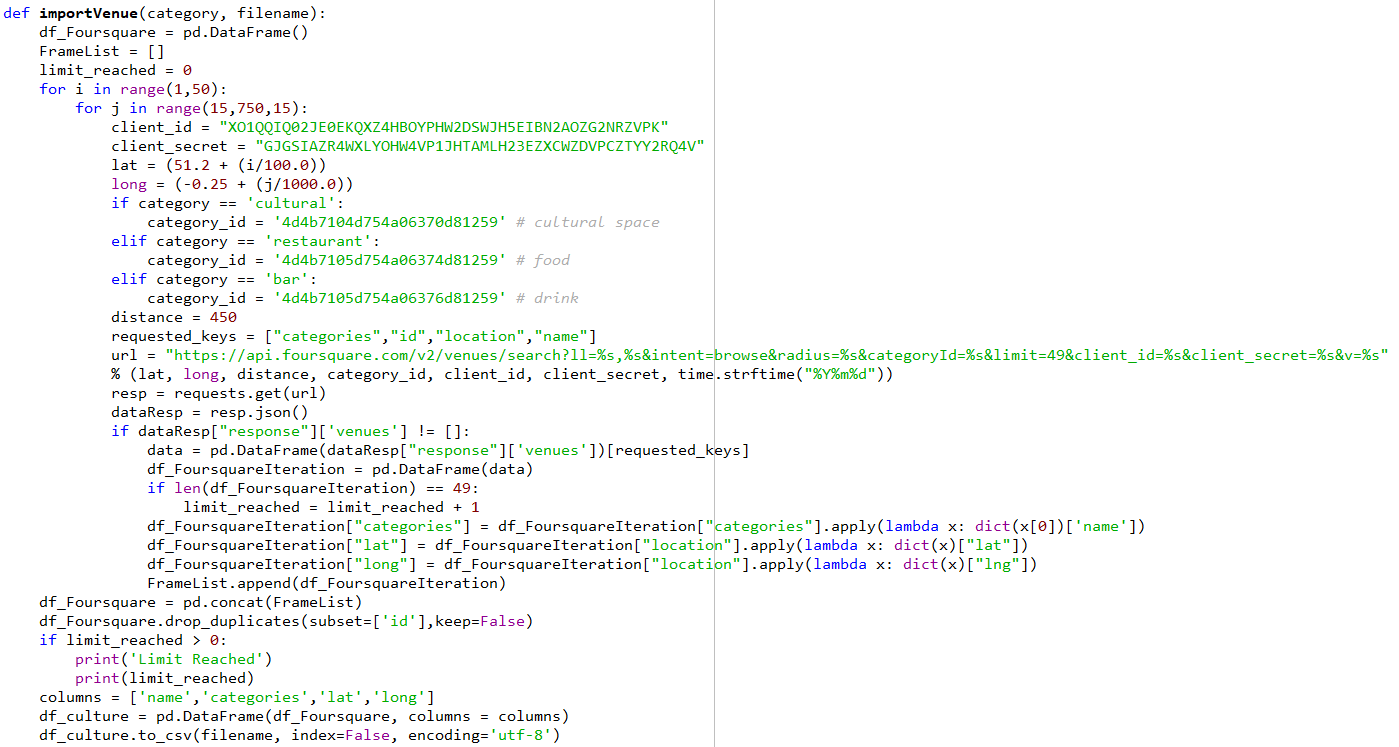
\includegraphics[scale=0.75]{figures/API_import} % Code example

Because of the rate limits, running the algorithm for such a large area could only be done on a daily basis.

%----------------------------------------------------------------------------------------
%	SECTION 2
%----------------------------------------------------------------------------------------

\section{Well-being domain scores}



%----------------------------------------------------------------------------------------
%	SECTION 3
%----------------------------------------------------------------------------------------

\section{London house prices as a regression problem}

London is known for having very high real estate values but we can see from the map below that there are specific wards, particularly in the western central area, where median house prices are significantly above the Greater London area as a whole.

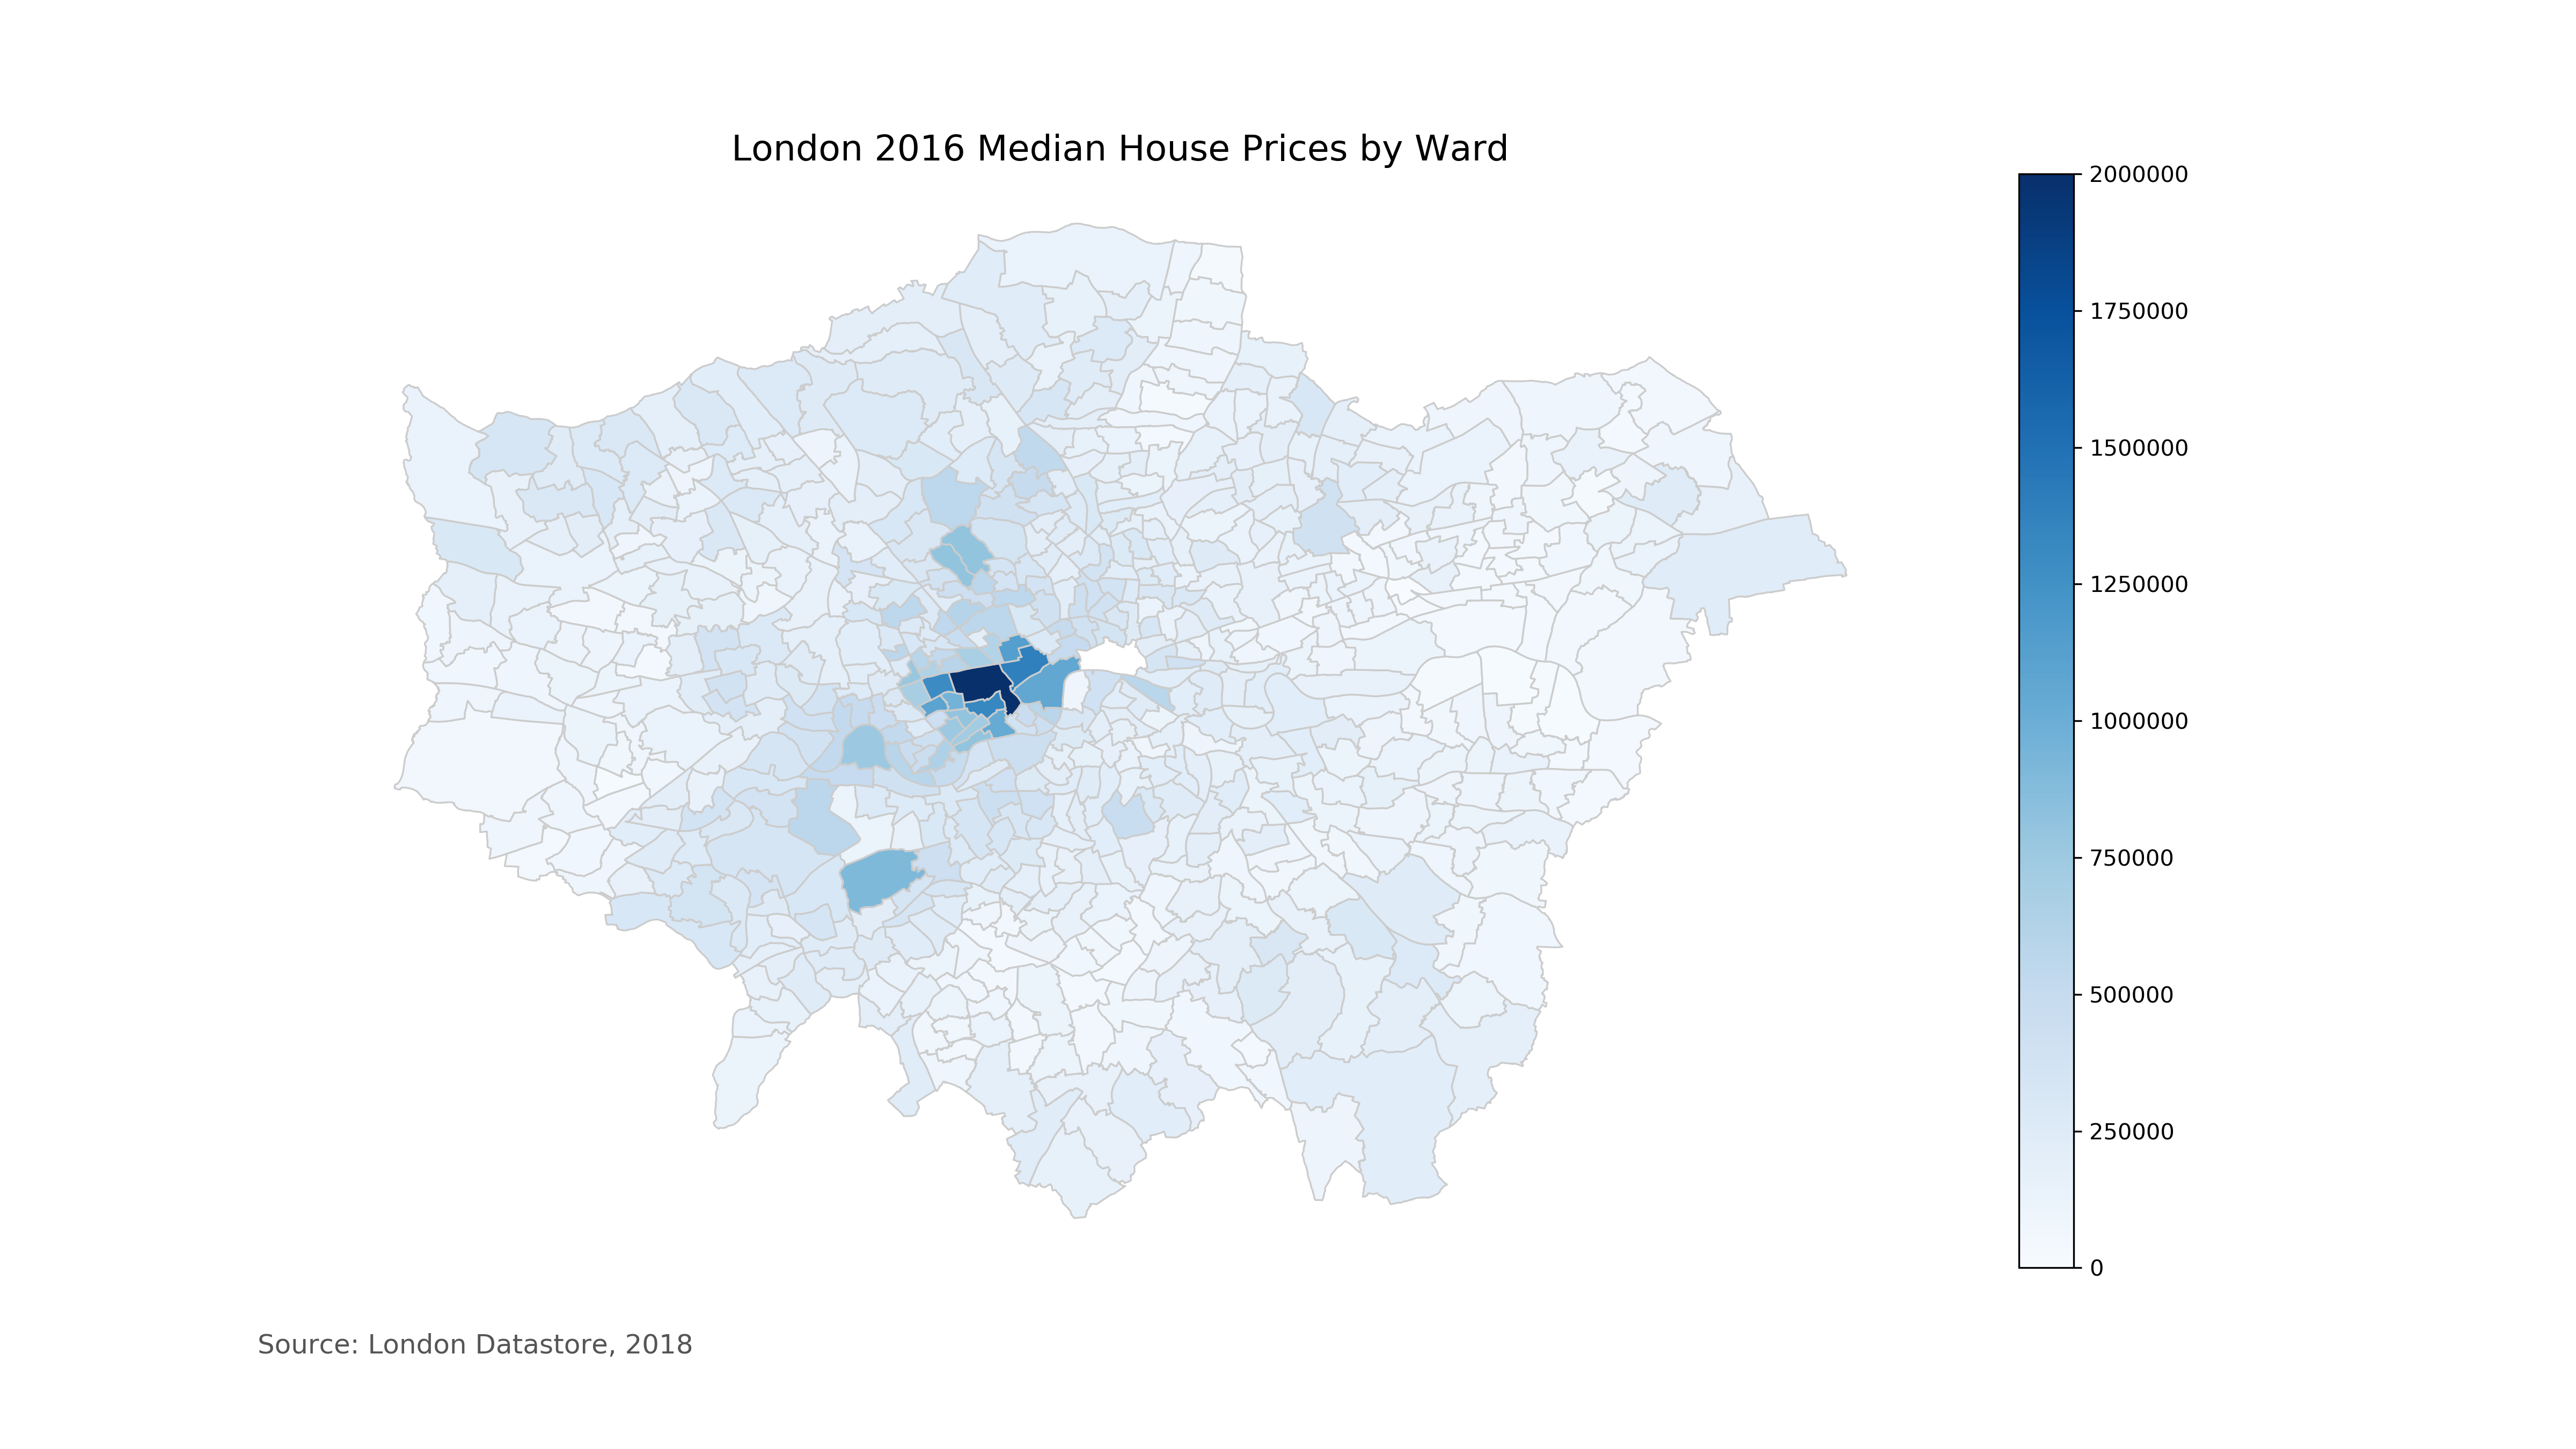
\includegraphics[scale=0.4]{figures/HPMedian} % Choropleth of median house prices


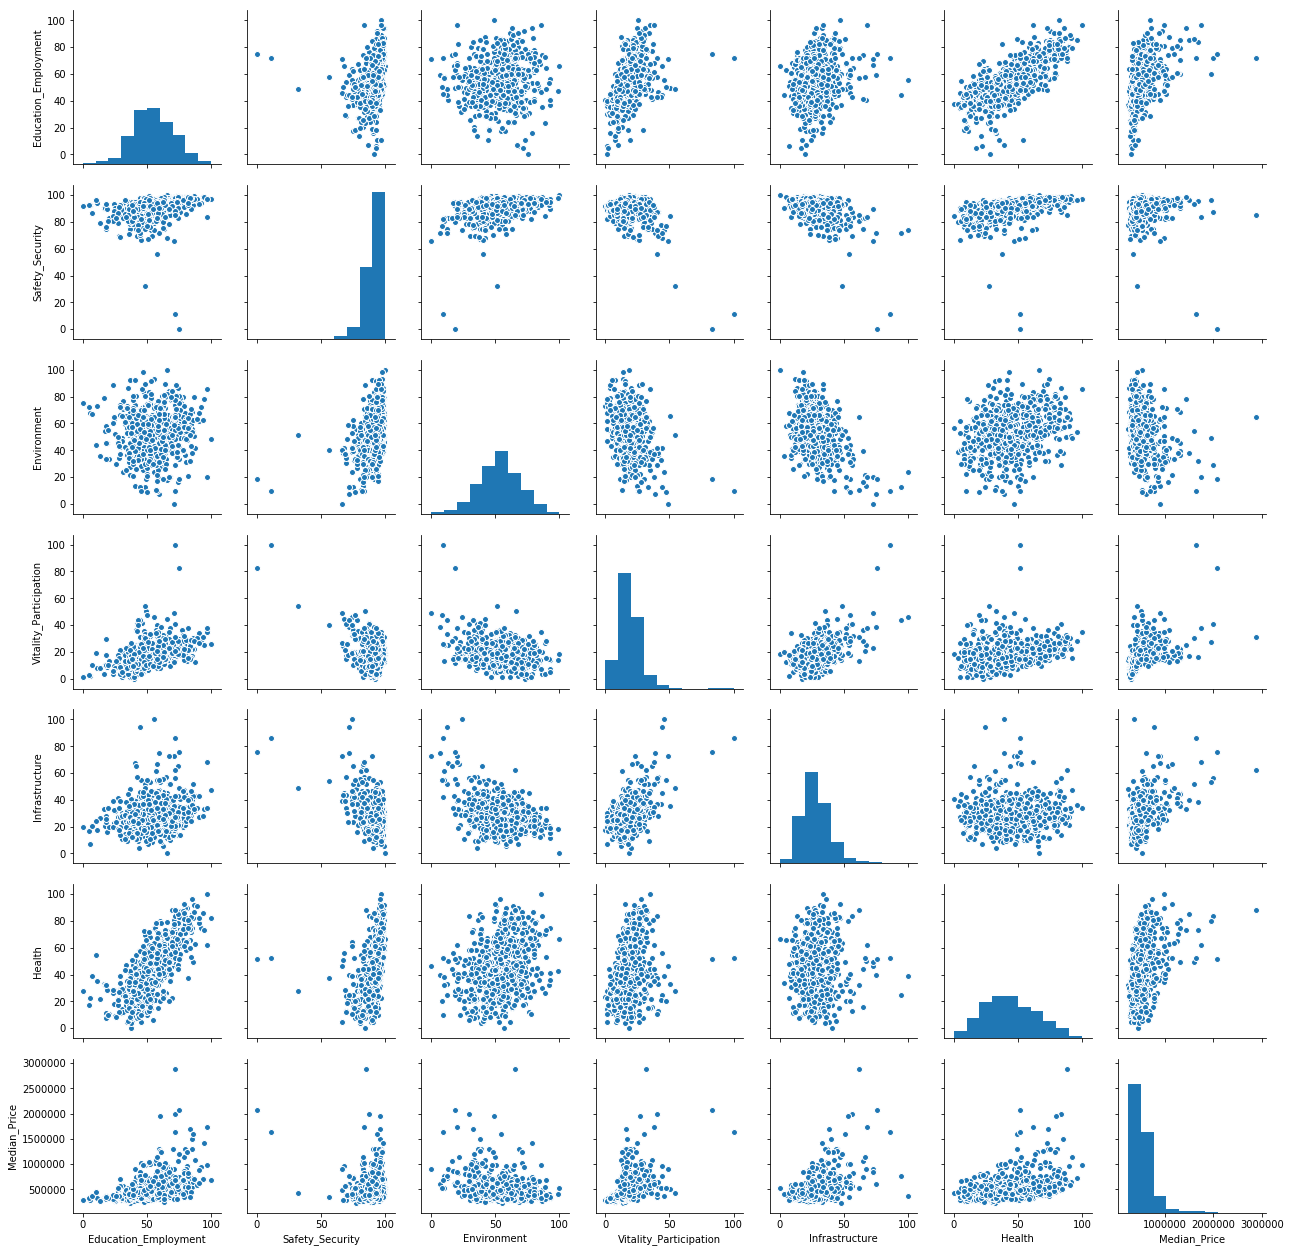
\includegraphics[scale=0.3]{figures/pairplot} % Pair-wise plot with median prices

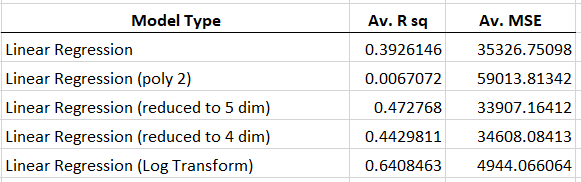
\includegraphics[scale=1]{figures/regression_results} % Pair-wise plot with median price

Looking at the median house prices on the pair-wise plot, the distribution looks as though it may be governed by a power law. On this basis, to try and improve the regression model I re-ran the regression model having log transformed the data. This lead to a signifcant increase in the Rsq score for the model, with an increase of around 0.45 to around 0.65 accounting for an additional 20 percent of the variation in the data. This was a far more effective strategy than using polynomial terms or dimension reduction and accounted for the best regression model. The equation given by this model was:

[insert model equation]

When the predictions were given the inverse transformation and compared with the actual values, the majority of wards showed that this model had good predictive capability although there were a handful of wards where the prediction had a signifcant error margin.  

%----------------------------------------------------------------------------------------
%	SECTION 4
%----------------------------------------------------------------------------------------

\section{London house prices as a classification problem}

Sed ullamcorper quam eu nisl interdum at interdum enim egestas. Aliquam placerat justo sed lectus lobortis ut porta nisl porttitor

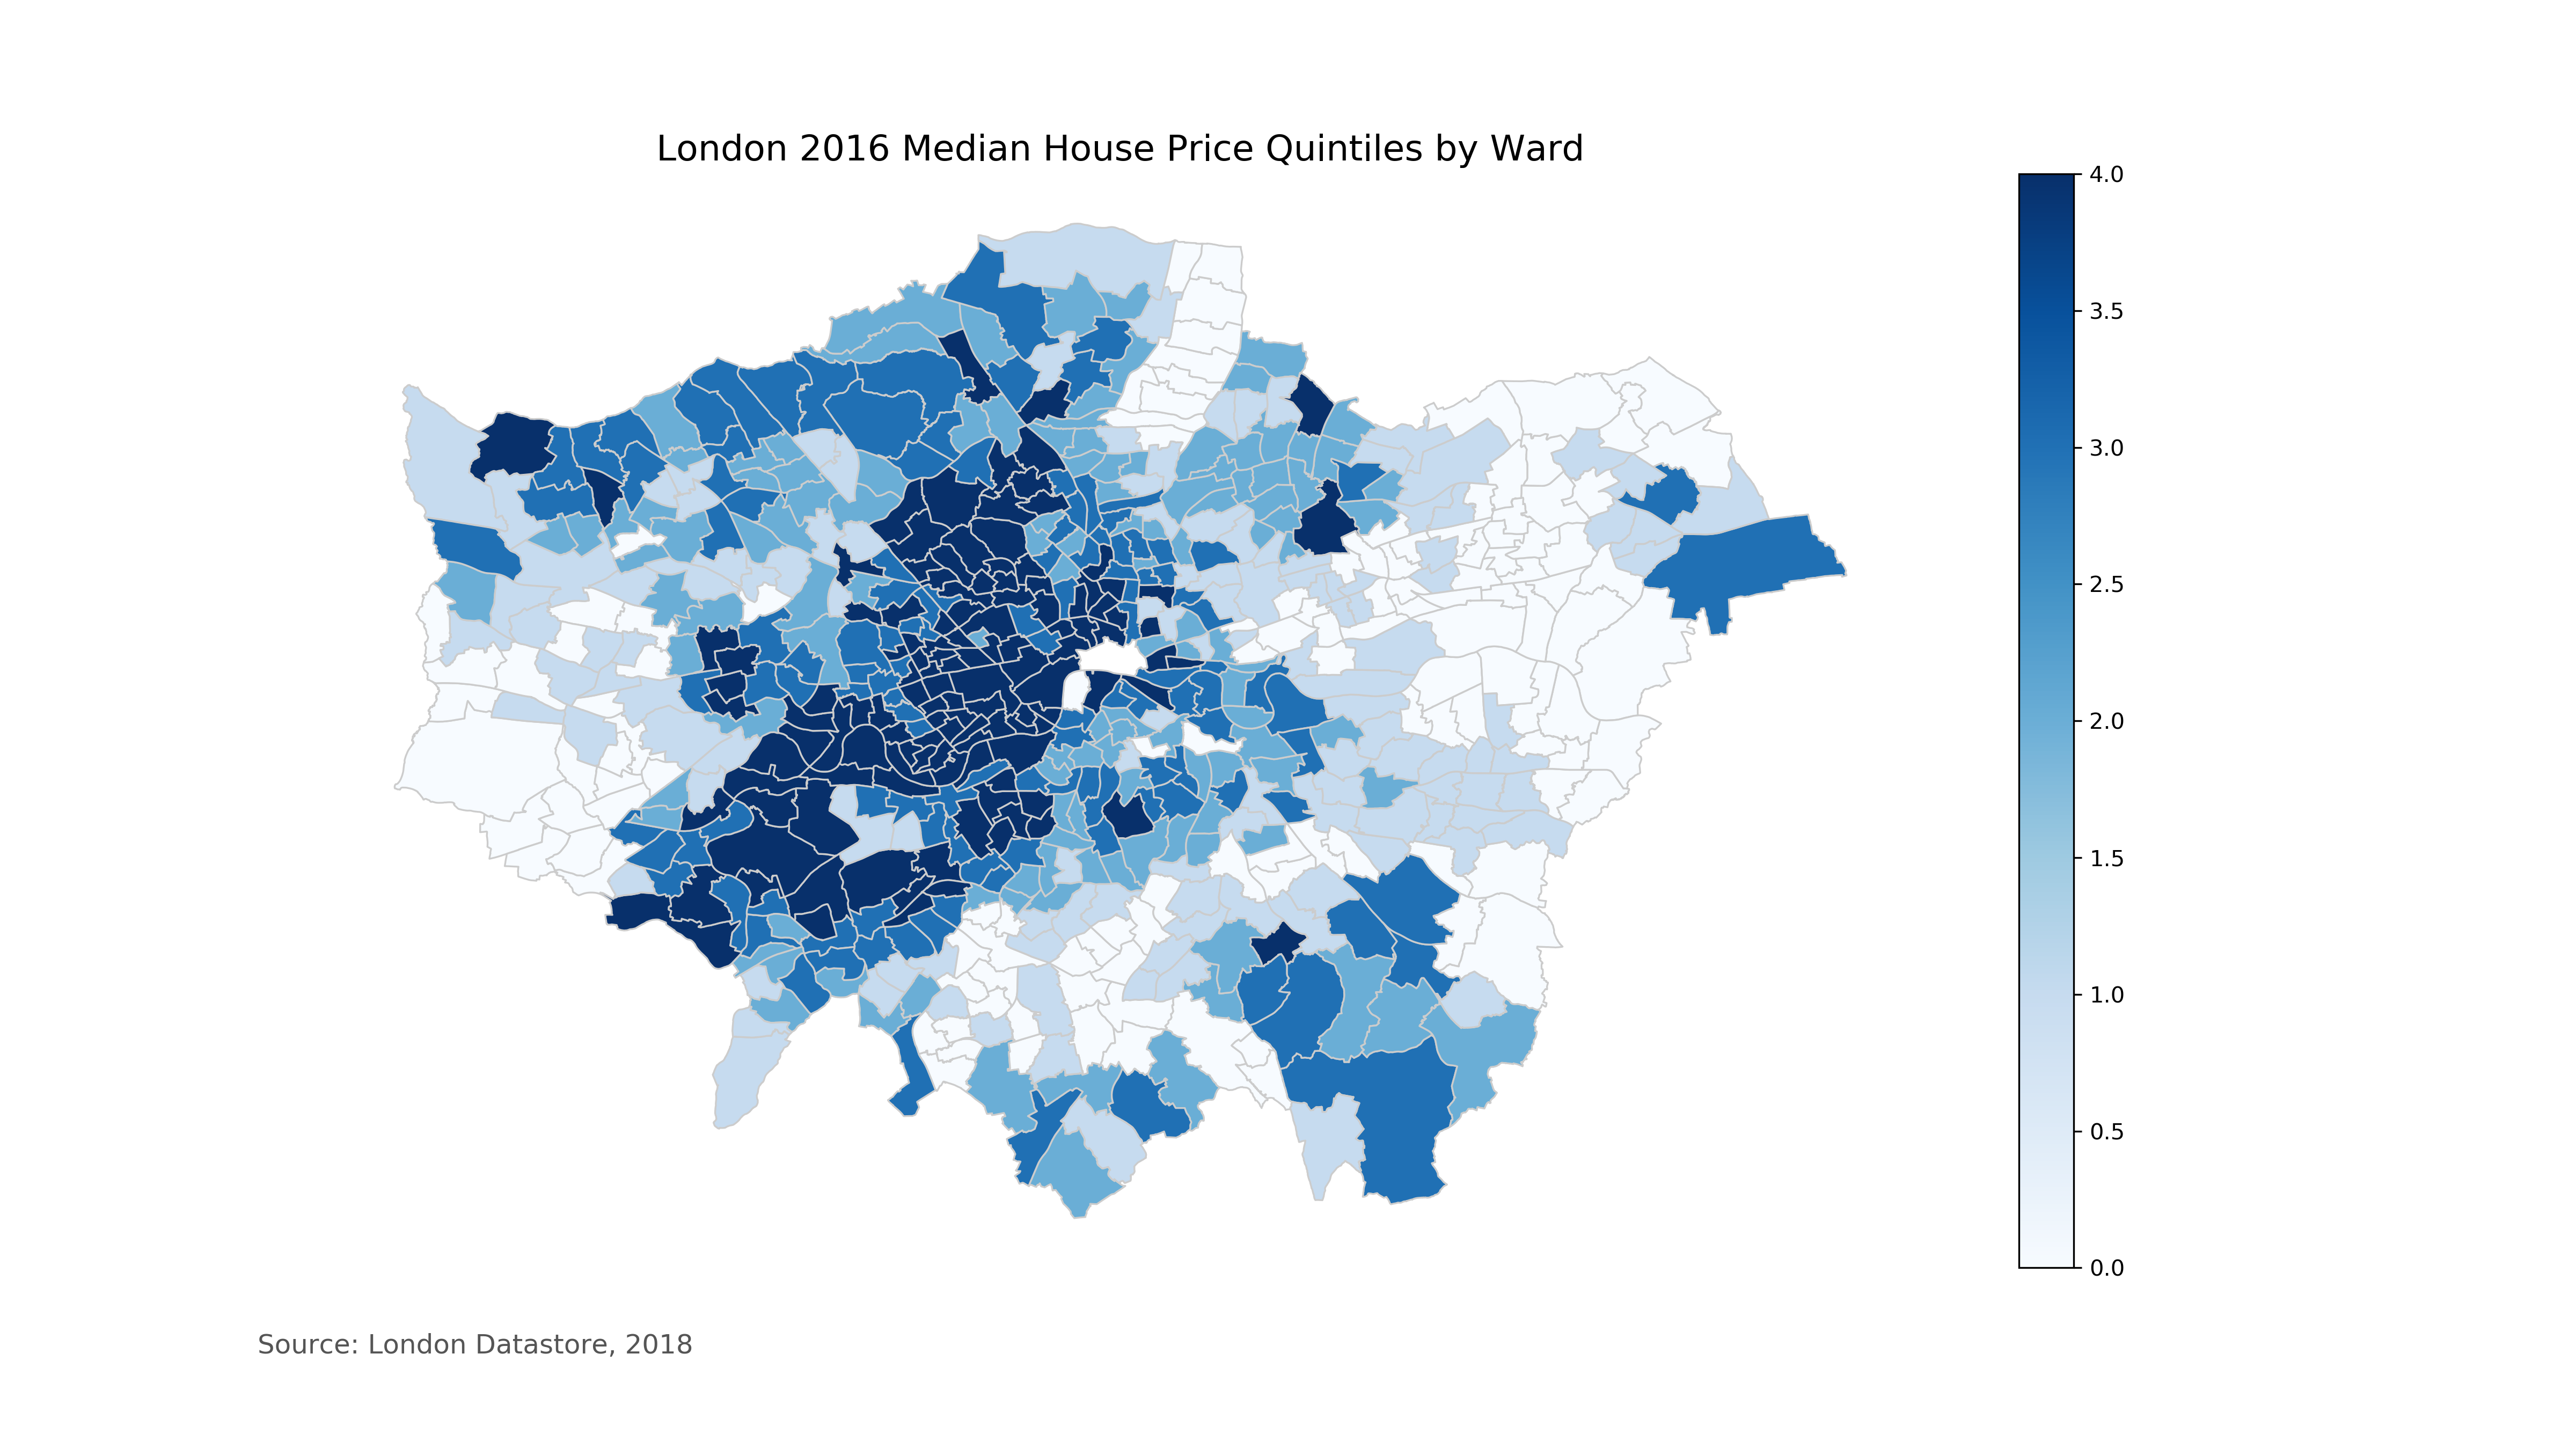
\includegraphics[scale=0.4]{figures/HPQuintile} % Choropleth of Median house prices by quintile

Sed ullamcorper quam eu nisl interdum at interdum enim egestas. Aliquam placerat justo sed lectus lobortis ut porta nisl porttitor

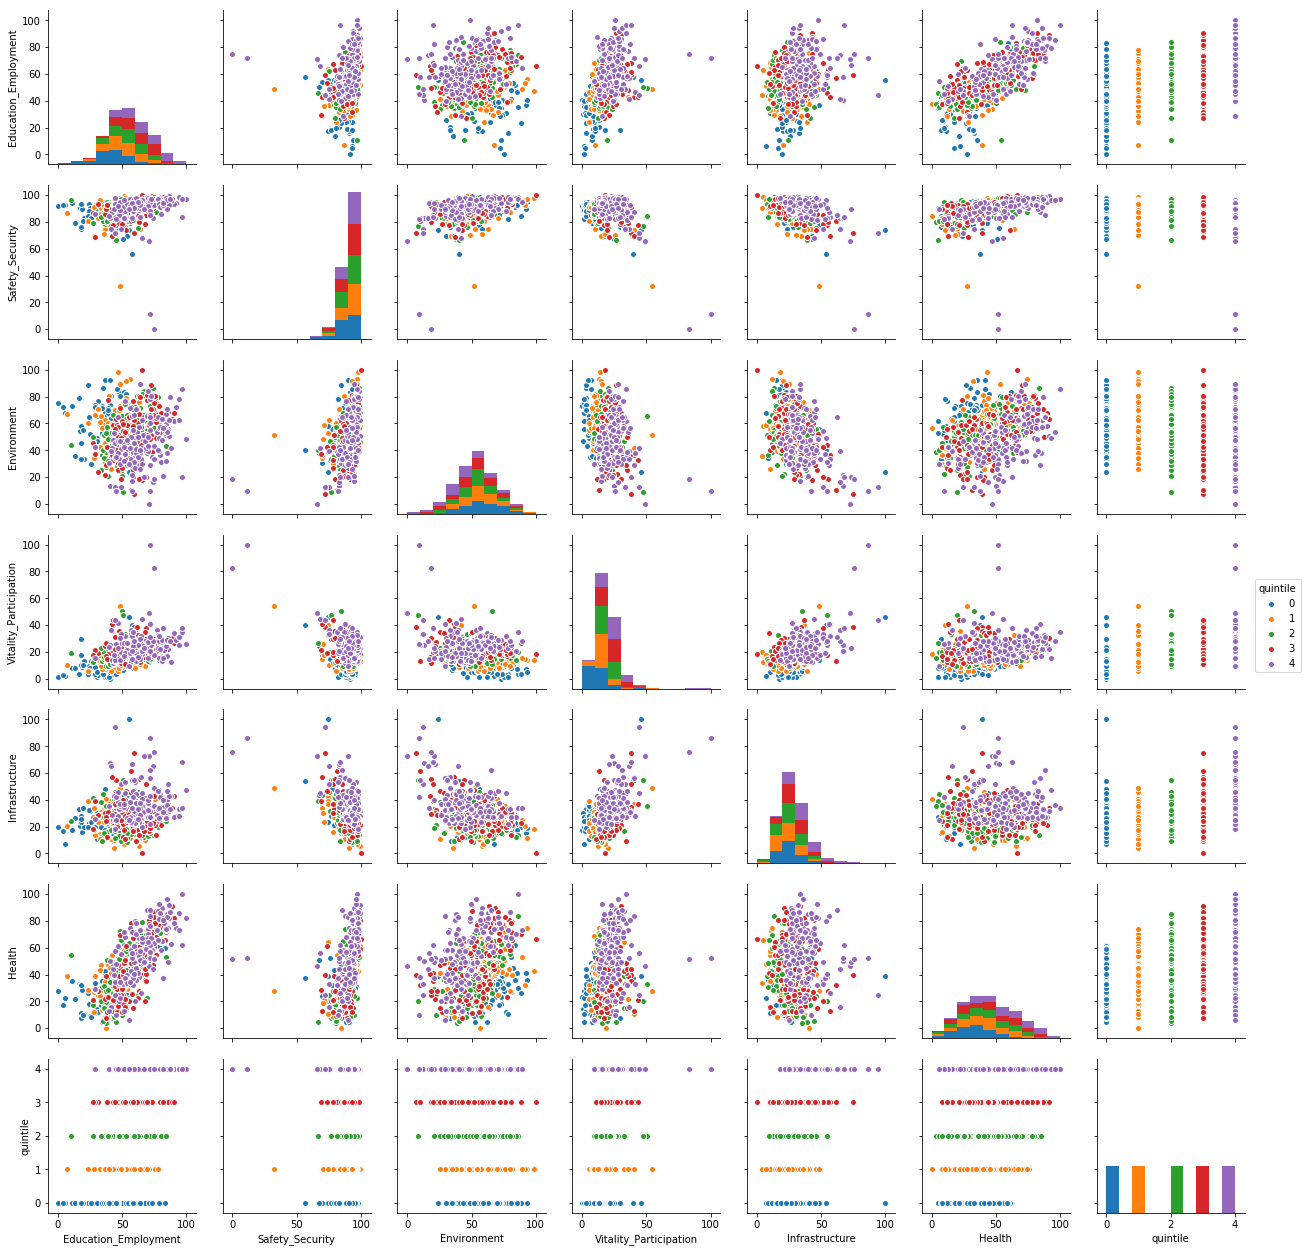
\includegraphics[scale=0.3]{figures/pairplot_quintile} % Pair-wise plot with median prices by quintile


%----------------------------------------------------------------------------------------
%	SECTION 5
%----------------------------------------------------------------------------------------

\section{Encoding as geoJSON}



%----------------------------------------------------------------------------------------
%	SECTION 6
%----------------------------------------------------------------------------------------

\section{Interactive maps}
